\documentclass[10pt, journal,compsoc]{article}
\usepackage{graphicx}
\usepackage{latexsym}
\usepackage{amsfonts}
\usepackage{listings}
\usepackage{mypriptrt} 

\begin{document}

\title{Neural Computation LU - Aufgabenblock 1 - Gruppe 8}


\author{Aitor Aldomà \and Thomas Kern \and Christian Weichselbaum}
        

\section{Exercise 1.1}
\subsection{Exercise 1.1.1}
\textit{Stellen Sie die Lage der Datenvektoren und ihre labels graphisch dar.}

\begin{figure}[htp]
	\centering
	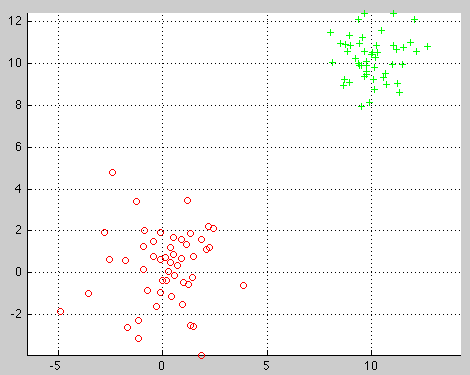
\includegraphics[width=1\textwidth]{ab1_1_1}
	\caption{Datensatz generiert mit genData(50,2)}\label{fig:1}
\end{figure}

\subsection{Exercise 1.1.2}

\textit{Untersuchen sie den Trainingsalgorithmus: Wieviele Iterationen wer den benötigt, bis sich weight-Vektor $w$ im Fall von linear separierbaren Daten nicht mehr andert?}
\\
8
\\
\\
\textit{Wie verändert sich der w während des Trainings?}
\\

\\
\\

\textit{Welchen Einfluss hat die Schrittweite?}
\\

\\
\\

\textit{Plotten Sie die Daten und Entscheidungsgrenze in $R^2$}
\\
\\
\\

\textit{Wie ist das Verhalten bei nicht linear separierbaren Daten?}

\subsection{Exercise 1.1.3}

\section{Exercise 1.2}
\subsection{Exercise 1.2.1}
asdf
\end{document}


